\def\year{2017}\relax
%File: formatting-instruction.tex
\documentclass[letterpaper]{article} %DO NOT CHANGE THIS
\usepackage{aaai18}  %Required
\usepackage{times}  %Required
\usepackage{helvet}  %Required
\usepackage{courier}  %Required
\usepackage{url}  %Required
\usepackage{graphicx}  %Required
\frenchspacing  %Required
\setlength{\pdfpagewidth}{8.5in}  %Required
\setlength{\pdfpageheight}{11in}  %Required
%PDF Info Is Required:
  \pdfinfo{}
\setcounter{secnumdepth}{0}

\usepackage{amsmath}
\usepackage{amssymb}
\usepackage{amsthm}
\usepackage{multirow}
\usepackage{tikz}
\usetikzlibrary{arrows,automata}
\usepackage{comment}

\usepackage{graphicx}
\usepackage{caption}
\usepackage{subcaption}
\usepackage{listings}

\lstset{
  basicstyle=\ttfamily,
  mathescape
}


\usepackage{multicol}
\usepackage{arydshln}
\usetikzlibrary{calc,backgrounds,positioning,fit}


\newcommand{\tup}[1]{{\langle #1 \rangle}}

\newcommand{\pre}{\mathsf{pre}}     % precondition
\newcommand{\del}{\mathsf{del}}     % effect
\newcommand{\add}{\mathsf{add}}     % effect
\newcommand{\eff}{\mathsf{eff}}     % effect
\newcommand{\cond}{\mathsf{cond}}   % conditional effect
\newcommand{\true}{\mathsf{true}}   % true
\newcommand{\false}{\mathsf{false}} % false
\newcommand{\PE}{\mathrm{PE}}     % precondition
\newcommand{\strips}{\textsc{Strips}}     % precondition


\newtheorem{theorem}{Theorem}
\newtheorem{lemma}[theorem]{Lemma}
\newtheorem{definition}[theorem]{Definition}


\begin{document}

\title{Model Recognition as Planning}

% Commented for blind submission
\author{Diego Aineto\and Sergio Jim\'enez\and Eva Onaindia \and Miquel Ram\'irez\\
{\small Departamento de Sistemas Inform\'aticos y Computaci\'on}\\
{\small Universitat Polit\`ecnica de Val\`encia.}\\
{\small Camino de Vera s/n. 46022 Valencia, Spain}\\
{\small \{dieaigar,serjice,onaindia\}@dsic.upv.es}}



\maketitle
\begin{abstract} 
Given the partial observation of a plan execution and a set of possible planning models (that share the same state variables but define different action models), {\em model recognition} is the task of identifying which model in the set explains (produced) the given observation. The paper formalizes the {\em model recognition} task and proposes a novel method to assess the probability of a \strips\ model to produce a partial observation of a plan execution. This method, that we called {\em model recognition as planning}, is built on top of off-the-shelf classical planning algorithms, that are used to elicit the likelihood of the observations given a candidate model. {\em Model recognition as planning} is robust to missing intermediate states and actions in the observed plan execution. The effectiveness of {\em model recognition as planning} is shown in a set of \strips\ models encoding different kinds of {\em finite state machines}. We show that {\em model recognition as planning} succeeds to identify the executed automata despite the internal machine state or actual applied transitions, are unobserved.
\end{abstract}

\section{Introduction}
\label{sec:introduction}
{\em Plan recognition} is the task of predicting the future actions of an agent provided observations of its current behavior. Plan recognition is considered {\em automated planning} in reverse; while automated planning aims to compute a sequence of actions that accounts for a given goals, plan recognition aims to compute the goals that account for an observed sequence of actions~\cite{geffner:book:2013}.

Diverse approaches has been proposed for plan recognition such as {\em rule-based systems}, {\em parsing}, {\em graph-covering}, {\em Bayesian nets}, etc~\cite{carberry2001techniques,sukthankar2014plan}. {\em Plan recognition as planning} is the model-based approach for plan recognition~\cite{ramirez2012plan,ramirez2009plan}. This approach assumes that the action model of the observed agent is known and leverages it to compute the most likely goal of the agent, according to the observed plan execution.

This paper introduces the {\em model recognition} task where the target of the recognition process is not a goal but a {\em planning model}. Given a partial observation of a plan execution and a set of possible planning models (that share the same state variables but define different action models), {\em model recognition} is the task of identifying which model in the set has the highest probability of producing the given observation.

\begin{figure}
  \begin{scriptsize}    
  \begin{center}
  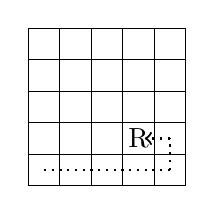
\begin{tikzpicture}[scale=.4]
          \begin{scope}
            \draw (0, 0) grid (5, 5);
            \node[anchor=center] at (3.5, 1.5) {R};
            \node[anchor=center] at (0.5, 0.5) {};
            \draw[thick,style=dotted] (0.5,0.5) -- (4.5,0.5);
            \draw[thick,style=dotted] (4.5,0.5) -- (4.5,1.5);
            \draw[thick,style=dotted,->] (4.5,1.5) -- (3.7,1.5);                        
          \end{scope}
        \end{tikzpicture}
\hspace*{1cm}        
	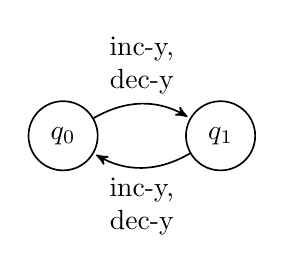
\begin{tikzpicture}[->,>=stealth',shorten >=1pt,auto,node distance=2cm,semithick]
	  \node[state] (A)              {$q_0$};
	  \node[state] (B) [right of=A] {$q_1$};          
	  \path
(A) edge [bend left, align=center] node {inc-y,\\dec-y} (B)
(B) edge [bend left, align=center] node {inc-y,\\dec-y} (A);
	\end{tikzpicture}
  \end{center}
  \end{scriptsize}  
 \caption{\small Observation of the execution of a robot navigation plan in a $5\times 5$ grid and a two state automata for controlling that the robot only increments its x-coordinate at {\em even} rows (i.e. at state $q_0$).}
\label{fig:grid-example}
\end{figure}

To better illustrate {\em model recognition}, imagine a robot in a $n\times n$ grid whose navigation is determined by the \strips\ model of Figure~\ref{fig:model-example}. According to this model the robot could increment its {\em x-coordinate} at {\em even} rows and decrement it at the {\em odd rows}. Apart from this particular navigation model, different models could be defined within the same state variables (e.g. altering the way {\small\tt (q0)} and {\small\tt (q1)} are required and updated) and these models can determine different kinds of robot navigation. Given an observation of a plan execution, like the one illustrated at Figure~\ref{fig:grid-example}, {\em model recognition} aims here to identify which navigation model produced that observation, despite key information is unobserved (e.g. the value of {\small\tt (q0)} and {\small\tt (q1)} or the particular applied actions). 

{\em Model recognition} is of interest because once the planning model is recognized, then the model-based machinery for automated planning becomes applicable~\cite{ghallab2004automated}. In addition, it enables identifying different kinds of automatae by observing their execution. It is well-known that diverse automatae representations, like {\em finite state controllers}, {\em push-down automata}, {\em {\sc GOLOG} programs} or {\em reactive policies}, can be encoded as classical planning models~\cite{baier2007exploiting,Geffner:FSM:AAAI10,ivankovic2015optimal,segovia2017generating}.

The paper introduces also {\em model recognition as planning}; a novel method to assess the probability of a given \strips\ model to produce an observed plan execution. Our method is built on top of off-the-shelf classical planning algorithms, that are used to elicit the likelihood of the observations given a candidate model. {\em Model recognition as planning} is robust to missing intermediate states and actions in the observed plan execution. We evaluate the effectiveness of {\em model recognition as planning} with a set of \strips\ models that represent different {\em finite state machines}. All of these {\em automatae} are defined within the same {\em alphabet} and same {\em machine states} but different {\em transition functions}. We show that {\em model recognition as planning} succeeds to identify the executed {\em automata} despite internal machine states or actual applied transitions are unobserved.

\begin{figure}
  \begin{tiny}
  \begin{verbatim}
  (:action inc-x
    :parameters (?v1 ?v2)
    :precondition (and (xcoord ?v1) (next ?v1 ?v2) (q0))
    :effect (and (not (xcoord ?v1)) (xcoord ?v2)))

  (:action dec-x
    :parameters (?v1 ?v2)
    :precondition (and (xcoord ?v1) (next ?v2 ?v1) (q1))
    :effect (and (not (xcoord ?v1)) (xcoord ?v2)))

  (:action inc-y-even
    :parameters (?y1 ?y2)
    :precondition (and (ycoord ?y1) (next ?y1 ?y2) (q0))
    :effect (and (not (ycoord ?y1)) (ycoord ?y2)
                 (not (q0)) (q1))

  (:action inc-y-odd
    :parameters (?y1 ?y2)
    :precondition (and (ycoord ?y1) (next ?y1 ?y2) (q1)))
    :effect (and (not (ycoord ?y1)) (ycoord ?y2)
                 (not (q1)) (q0)))

  (:action dec-y-even
    :parameters (?y1 ?y2)
    :precondition (and (ycoord ?y1) (next ?y2 ?y1) (q0))
    :effect (and (not (ycoord ?y1)) (ycoord ?y2)
                 (not (q0)) (q1)))

  (:action dec-y-odd
    :parameters (?y1 ?y2)
    :precondition (and (ycoord ?y1) (next ?y2 ?y1) (q1))
    :effect (and (not (ycoord ?y1)) (ycoord ?y2)
                 (not (q1)) (q0)))
  \end{verbatim}           
  \end{tiny}  
 \caption{\small Action model for a robot navigation in a $n\times n$ grid.}
\label{fig:model-example}
\end{figure}



\section{Background}
\label{sec:background}
This section formalizes the models for {\em classical planning} and for the {\em observations} of a plan execution.

\subsection{Classical planning}
We use $F$ to denote the set of {\em fluents} (propositional variables) describing a state. A {\em literal} $l$ is a valuation of a fluent $f\in F$, i.e. either~$l=f$ or $l=\neg f$. A set of literals $L$ represents a partial assignment of values to fluents (without loss of generality, we will assume that $L$ does not assign conflicting values to any fluent). We use $\mathcal{L}(F)$ to denote the set of all literal sets on $F$, i.e.~all partial assignments of values to fluents.

A {\em state} $s$ is a full assignment of values to fluents and we explicitly include negative literals $\neg f$ in states; i.e. $|s|=|F|$, so the size of the state space is $2^{|F|}$. Like in PDDL~\cite{fox2003pddl2}, we assume that fluents $F$ are instantiated from a set of {\em predicates} $\Psi$. Each predicate $p\in\Psi$ has an argument list of arity $ar(p)$. Given a set of {\em objects} $\Omega$, the set of fluents $F$ is induced by assigning objects in $\Omega$ to the arguments of predicates in $\Psi$; i.e.~$F=\{p(\omega):p\in\Psi,\omega\in\Omega^{ar(p)}\}$ such that $\Omega^k$ is the $k$-th Cartesian power of $\Omega$.

A {\em classical planning frame} is a pair $\tup{F,A}$, where $F$ is a set of fluents and $A$ is a set of actions whose semantics are specified with two functions: $\rho(s,a)$ that denotes whether an action $a\in A$ is {\em applicable} in a state $s$ and $\theta(s,a)$ that denotes the {\em successor state} that results of applying $a$ in $s$. In this work we specify action semantics with the \strips\ model. With this regard, an action $a\in A$ is defined with:
\begin{itemize}
\item $\pre(a)\in\mathcal{L}(F)$, the {\em preconditions} of $a$, is the set of literals that must hold for the action $a\in A$ to be applicable.
\item $\eff^+(a)\in\mathcal{L}(F)$, the {\em positive effects} of $a$, is the set of literals that are true after the application of action $a\in A$.
\item $\eff^-(a)\in\mathcal{L}(F)$, the {\em negative effects} of $a$, is the set of literals that are false after the application of the action.
\end{itemize}
We say that an action $a\in A$ is {\em applicable} in a state $s$ iff $\pre(a)\subseteq s$. The result of applying $a$ in $s$ is the {\em successor state} denoted by $\theta(s,a)=\{s\setminus\eff^-(a))\cup\eff^+(a)\}$.

A {\em classical planning problem} is a tuple $P=\tup{F,A,I,G}$, where $I$ is an initial state and $G\in\mathcal{L}(F)$ is a goal condition. A {\em plan} $\pi$ for $P$ is an action sequence $\pi=\tup{a_1, \ldots, a_n}$ that induces the {\em state trajectory} $s=\tup{s_0, s_1, \ldots, s_n}$ such that $s_0=I$ and, for each {\small $1\leq i\leq n$}, $a_i$ is applicable in $s_{i-1}$ and generates the successor state $s_i=\theta(s_{i-1},a_i)$. The {\em plan length} is denoted with $|\pi|=n$ . A plan $\pi$ {\em solves} $P$ iff $G\subseteq s_n$, i.e.,~if the goal condition is satisfied at the last state reached after following the application of the plan $\pi$ in the initial state $I$. A solution plan for $P$ is {\em optimal} if it has minimum length.

\subsection{Conditional effects}
{\em Conditional effects} allow planning actions to have different semantics according to the value of the current state. This feature is useful for compactly defining our method for {\em model recognition as planning}. 

An action $a\in A$ with conditional effects is defined as a set of {\em preconditions} $\pre(a)\in\mathcal{L}(F)$ and a set of {\em conditional effects} $\cond(a)$. Each conditional effect $C\rhd E\in\cond(a)$ is composed of two sets of literals $C\in\mathcal{L}(F)$, the {\em condition}, and $E\in\mathcal{L}(F)$, the {\em effect}.

An action $a\in A$ is {\em applicable} in a state $s$ iff $\pre(a)\subseteq s$, and the {\em triggered effects} resulting from the action application are the effects whose conditions hold in $s$:
\[
triggered(s,a)=\bigcup_{C\rhd E\in\cond(a),C\subseteq s} E,
\]

The result of applying action $a$ in state $s$ is the {\em successor} state $\theta(s,a)=\{s\setminus\eff_c^-(s,a))\cup\eff_c^+(s,a)\}$ where $\eff_c^-(s,a)\subseteq triggered(s,a)$ and $\eff_c^+(s,a)\subseteq triggered(s,a)$ are, respectively, the triggered {\em negative} and {\em positive} effects.

\subsection{The observation model}
Given a classical planning problem $P=\tup{F,A,I,G}$ and a plan $\pi$ that solves $P$, the observation of the execution of  $\pi$ on $P$ is $\tau=\tup{a_1^o, \ldots , a_n^o, s_m^o}$, an interleaved combination of {\small $1\leq n\leq |\pi|$} observed actions and {\small $1\leq m\leq |\pi|+1$} observed states such that:
\begin{itemize}
\item Observed actions are {\em consistent} with $\pi$~\cite{ramirez2009plan}. This means that the sequence of observed actions $\tup{a_1^o, \ldots, a_n^o}$ in $\tau$ is a sub-sequence of the solution plan $\pi$.
\item Observed states are a sub-sequence  of partial states that is {\em consistent} with the sequence of states traversed by $\pi$. 
\end{itemize}

On the one hand, the initial state $I$ is fully observed while the observed states in $\tau$ may be partial, i.e. the value of certain fluents in the intermediate states may be omitted (~$|s_i^o|\leq |F|$ for every $1\leq i\leq m$). On the other hand, the sequence of observed states $\tup{s_1^o, \ldots, s_m^o}$ in $\tau$ is the same sequence of states traversed by $\pi$ but certain states may also be omitted. Formally, $0\leq|s_i^o|$ for every $1\leq i\leq m$. This means that the transitions between two consecutive observed states in $\tau$ may require the execution of more than a single action ($\theta(s_i^o,\tup{a_1,\ldots,a_k})=s_{i+1}^o$, where $k\geq 1$ is unknown and unbound). Therefore we can conclude that having $\tau$ does not implies knowing the actual length of $\pi$.

\begin{definition}[$\Phi$-observation]
Given a subset of fluents $\Phi\subseteq F$ we say that $\tau$ is a $\Phi$-observation of the execution of $\pi$ on $P$ iff, for every $0\leq i\leq m$, each observed state $s_i^o$ only contains fluents in $\Phi$.
\end{definition}

For instance, Figure~\ref{fig:grid-example} illustrates the $\Phi$-observation \{{\tt\scriptsize<(xcoord 1)(ycoord 1)>, <(xcoord 2)(ycoord 1)>, <(xcoord 3)(ycoord 1)>, <(xcoord 4)(ycoord 1)>, <(xcoord 5)(ycoord 1)>, <(xcoord 5)(ycoord 2)>, <(xcoord 4)(ycoord 2)>}\} where $\Phi$ only contains fluents of the kind {\tt\small (xcoord ?v)} and {\tt\small (ycoord ?v)}. This means that, for each observed state, only the value of fluents {\tt\small (xcoord ?v)} and {\tt\small (ycoord ?v)} is known while the value of the fluents {\tt\small (next ?v1 ?v2)}, {\tt\small (q0)} and {\tt\small (q1)} is unknown.



\section{Model Recognition}
\label{sec:recognition}
The {\em model recognition} task is a tuple $\tup{P,M,\tau}$ where:
\begin{itemize}
\item $P=\tup{F,A,I,G}$ is a {\em classical planning problem} such that the semantics of the actions in $A$ is unknown because functions $\rho(s,a)$ and/or $\theta(s,a)$ are undefined.
\item $M=\{\mathcal{M}_1,\ldots,\mathcal{M}_m\}$ is a finite and non-empty {\em set of models} for the actions in $A$ such that, each model in $\mathcal{M}\in M$, defines a different function pair $\tup{\rho,\theta}$.
\item $\tau$ is an {\em observation} of the execution of a solution plan $\pi$ for $P$.
\end{itemize}

In the {\em model recognition} task, hypotheses are about the possible action models $\mathcal{M}\in M$ while $\tau$ represents the given observation. The {\em discrete probability distribution} $P(\mathcal{M}|\tau)$ expresses, for each model $\mathcal{M}\in M$, its probability of producing the input observation. According to the {\em Bayes rule} this probability distribution is given by $P(\mathcal{M}|\tau)=\frac{P(\tau|\mathcal{M})P(\mathcal{M})}{P(\tau)}$ and can be estimated in these three steps:
\begin{enumerate}
\item Estimating the {\em a priori probabilities} (if they are not already given as input). $P(\tau)$, that measures how surprising is the given observation and $P(\mathcal{M})$, that expresses if one model is known to be a priori more likely than the others. 
\item Computing likelihoods $P(\tau|\mathcal{M})$.  Our approach is to estimate these likelihoods according to the {\em amount of edits} required by the model $\mathcal{M}$ to produce a plan $\pi$ such that:
\begin{enumerate}
\item $\pi$ solves $P$ and,
\item $\tau$ is a consistent observation of the execution of $\pi$ on the classical planning problem $P$. 
\end{enumerate}
The {\em edit distance} is a similarity metric that is traditionally computed over {\em strings} or {\em graphs} and that has been proved successful for {\em pattern recognition}~\cite{masek1980faster,bunke1997relation}. In this work this similarity metric refers to the edition of classical planning models.
\item Applying the {\em Bayes rule} to obtain the normalized posterior probabilities. The $P(\mathcal{M}|\tau)$ probabilities must sum 1 for all the $\mathcal{M}\in M$.
\end{enumerate}

The {\em naive Bayes classifier} assigns a model $\mathcal{M}\in M$ to the given observation $\tau$ wrt the following expression, $argmax_{\mathcal{M}\in M} P(\mathcal{M})\times P(\tau|\mathcal{M})$. The {\em solution} to the {\em model recognition} task is the model $\mathcal{M}\in M$ (or subset of models in $M$) that maximizes the previous expression.



\section{Recognition of \strips\ models}
\label{sec:asPlanning}
Here we analyze the particular instantiation of the {\em model recognition} task where the semantics of actions (in other words, the corresponding $\rho$ and $\theta$ functions) are specified with \strips\ action schemas.

We start formalizing the \strips\ schema and define then the full space of possible \strips\ schema. Eventually, we introduce an {\em edit distance} for \strips\ schema which allows us to estimate the $P(\tau|\mathcal{M})$ likelihoods for planning models.

\subsection{Well-defined \strips\ action schema}
\strips\ action schema provide a compact representation for specifying classical planning models. For instance, Figure~\ref{fig:model-example} shows six \strips\ action schema, codded in PDDL, that determine a robot navigation in a $n\times n$ grid.

A \strips\ action schema $\xi$ is defined by a list of {\em parameters} $pars(\xi)$, and the three list of predicates ($pre(\xi)$, $del(\xi)$ and $add(\xi)$) that shape the kind of fluents that can appear in the {\em preconditions}, {\em negative effects} and {\em positive effects} of the actions induced from the schema. 

Given a \strips\ action schema $\xi$, let us define an additional set of objects ($\Omega\cap\Omega_\xi=\emptyset$), that we denote as {\em variable names}, and that contains one variable name for each parameter in $pars(\xi)$, that is $\Omega_\xi=\{v_i\}_{i=1}^{|pars(\xi)|}$. Note that, for any of the actions schema defined in~\ref{fig:model-example}, $\Omega_\xi=\{v_1,v_2\}$.

The set of FOL interpretations of $\Psi$ (the {\em predicates} that shape the propositional state variables) over the corresponding $\Omega_\xi$ objects (the {\em variable names} for that schema), confines the elements that can appear in the $\xi$ \strips\ action schema, that is in each of its $pre(\xi)$, $del(\xi)$ and $add(\xi)$ lists. We denote this set of FOL interpretations as ${\mathcal I}_{\Psi,\xi}$. For any of the actions schema defined in~\ref{fig:model-example} this set contains the same ten elements, ${\mathcal I}_{\Psi,\xi}=${\small\tt\{xcoord($v_1$), xcoord($v_2$), ycoord($v_1$), ycoord($v_2$), q0(), q1(), next($v_1$,$v_1$), next($v_1$,$v_2$), next($v_2$,$v_1$), next($v_2$,$v_2$))\}}.

Despite any element from ${\mathcal I}_{\Psi,\xi}$ can {\em a priori} appear in the $pre(\xi)$, $del(\xi)$ and $add(\xi)$ lists of a schema $\xi$. The space of possible \strips\ schema for $\xi$ is bound further by a set of constraints ${\mathcal C}$ of the following three kinds: 
\begin{itemize}
\item {\em Syntactic constraints}. \strips\ constraints require negative effects appearing as preconditions, negative effects cannot be positive effects at the same time and also, positive effects cannot appear as preconditions. Formally, $\eff^-(a)\subseteq \pre(a)$, $\eff^-(a)\cap \eff^+(a)=\emptyset$ and $\pre(a)\cap \eff^+(a)=\emptyset$). Given exclusively these syntactic constraints, the size of the space of possible \strips\ schema is given by the expression, $2^{2\times|{\mathcal I}_{\Psi,\xi}|}$. For the navigation model of Figure~\ref{fig:model-example}, $2^{2\times 10}=1,048,576$ for every action schema.
\item {\em Domain-specific constraints}. One can also introduce domain-specific knowledge to more precisely bound the space of possible \strips\ schema for a particular domain. For instance, in a {\em robot navigation} model, like the one in Figure~\ref{fig:model-example}, predicates {\small\tt q0()} and {\small\tt q1()} are always exclusive so they cannot hold a the same time in the $pre(\xi)$, $del(\xi)$ and $add(\xi)$ lists. Further, {\small\tt next($v_1$,$v_1$)} and {\small\tt next($v_2$,$v_2$)} will not appear at any of these lists because the {\tt\small next} predicate is coding the {\em succesor} function for {\em natural numbers}. In this case, introducing this domain-specific constraints would reduce the size of the space of possible schema to $2^{2\times 7}=16384$, for every action schema.
\end{itemize}

Now we are ready to define what is a well-defined \strips\ action schema.
\begin{definition}[Well-defined \strips\ action schema]
Given a set of {\em predicates} $\Psi$, a list of action {\em parameters} $pars(\xi)$, and set of FOL constraints ${\mathcal C}$ we say that $\xi$ is a {\bf well-defined \strips\ action schema} iff its three lists $pre(\xi)\subseteq {\mathcal I}_{\Psi,\xi}$, $del(\xi)\subseteq{\mathcal I}_{\Psi,\xi}$ and $add(\xi)\subseteq{\mathcal I}_{\Psi,\xi}$ only contain elements in ${\mathcal I}_{\Psi,\xi}$ and they satisfy all the constraints in ${\mathcal C}$. 
\end{definition}

\subsection{The \strips\ edit distance}
We define two edit \emph{operations} on a schema $\xi\in\mathcal{M}$ that belongs to a \strips\ action model $\mathcal{M}\in M$:
\begin{itemize}
\item {\em Deletion}. An element in ${\mathcal I}_{\Psi,\xi}$ is removed from any of these three lists $pre(\xi)$, $del(\xi)$ and $add(\xi)$ of the operator schema $\xi\in\mathcal{M}$ such that the resulting schema is a {\em well-defined} \strips\ action schema.
\item {\em Insertion}. An element in ${\mathcal I}_{\Psi,\xi}$ is added to any of these three lists $pre(\xi)$, $del(\xi)$ and $add(\xi)$ of the operator schema $\xi\in\mathcal{M}$ s.t. the resulting schema is {\em well-defined}.
\end{itemize}

We can now formalize an {\em edit distance} that quantifies how similar two given \strips\ action models are. The distance is symmetric and meets the {\em metric axioms} provided that the two {\em edit operations}, deletion and insertion, have the same positive cost.

\begin{definition}[Edit distance]
  Let $\mathcal{M}$ and $\mathcal{M}'$ be two {\em comparable} \strips\ action models defined within the same set of predicates $\Psi$. The {\bf edit distance} $\delta(\mathcal{M},\mathcal{M}')$ is the minimum number of {\em edit operations} that is required to transform $\mathcal{M}$ into $\mathcal{M}'$.
\end{definition}

Since ${\mathcal I}_{\Psi,\xi}$ are bound sets, the maximum number of edits that can be introduced to a given action model is bound as well. 
\begin{definition}[Maximum edit distance]
The \textbf{maximum edit distance} of an \strips\ model $\mathcal{M}$ built within the set of predicates $\Psi$ is $\delta(\mathcal{M},*)=\sum_{\xi\in\mathcal{M}} 3\times|{\mathcal I}_{\Psi,\xi}|$.
\end{definition}

The observation of plan executions that are generated with $\xi$ action schema constrain further the space of possible schema. In this case we talk about {\em semantic constraints} that can also be added the $\mathcal{C}$ set. We define now an edit distance to asses the matching of a \strips\ model with respect to an observation of a plan execution. 

\begin{definition}[Observation edit distance]
  Given $\tau$, an observation of the execution of a plan for solving $P$ and a \strips\ action model $\mathcal{M}$, all defined within the same set of predicates $\Psi$. The {\bf observation edit distance}, $\delta(\mathcal{M},\tau)$, is the minimal edit distance from $\mathcal{M}$ to any {\em comparable} model $\mathcal{M}'$ s.t. $\mathcal{M}'$ produces a plan $\pi^*_\tau$ optimal for $P$ and compliant with $\tau$; \[\delta(\mathcal{M},\tau)=\min_{\forall \mathcal{M}' \rightarrow \tau} \delta(\mathcal{M},\mathcal{M}')\]
\end{definition}

Remarkably, the {\em observation edit distance} allows us to elicit the likelihood of the observations given a candidate model. It can be argued that the shorter this  distance the better the given model explains the given observation and hence, the higher the likelihood $P(\tau|\mathcal{M})$. In particular this distance is maximum when it requires fully editing all the schemas in the model while it is minimum when the given model can produce the input observation without introducing any change. Intermmediate distance values reflect how far are the models from explaining the input observations. In this work we map the {\em observation edit distance} into a likelihood with the following expression $P(\tau|\mathcal{M}) = 1-\frac{\delta(\mathcal{M},\tau)}{\delta(\mathcal{M},*)}$.

Note that the {\em observation edit distance} could also be defined assessing the edition required by the observed plan execution to match the given model. This implies defining {\em edit operations} that modify $\tau$ instead of $\mathcal{M}$~\cite{sohrabi:precognition:IJCAI2016}. Our definition of the {\em observation edit distance} is more practical since normally ${\mathcal I}_{\Psi,\xi}$ is much smaller than $F$. In practice, the number of {\em variable objects} should be smaller than the number of objects in a planning problem.





\section{Model recognition with classical planning}
This section shows that, when the dynamics of the actions $A\in P$ are specified with \strips\ action schemas, then $\delta(\mathcal{M},\tau)$ can be computed with a compilation of a classical planning with conditional effects. The intuition behind this compilation is that a solution to the resulting classical planning task is a sequence of actions that:
\begin{enumerate}
\item {\bf Edits the action model $\mathcal{M}$ to build $\mathcal{M}'$}. A solution plan starts with a {\em prefix} that modifies the preconditions and effects of the action schemes in $\mathcal{M}$ using to the two {\em edit operations} defined above, {\em deletion} and {\em insertion}. 
\item {\bf Validates the edited model $\mathcal{M}'$}. The solution plan continues with a postfix that:
\begin{enumerate}
\item Induces an optimal solution plan $\pi^*_\tau$ for the original classical planning problem $P$.
\item Validates that $\tau$ is an observation of the execution of $\pi^*_\tau$ on the classical planning problem $P$.
\end{enumerate}
\end{enumerate}

Figure~\ref{fig:plan-pdistance} shows the plan with a prefix (steps [0,1]) for editing a given {\em blockswold} model where the positive effects {\tt\small (handempty)} and {\tt\small (clear ?v1)} of the {\tt\small stack} schema are missing. The postfix of the plan (steps [2,6]) validates the edited action model at the observation of a four action plan for inverting a two-block tower where intermediate states, $s_1$, $s_2$ and $s_3$, are unobserved. 
\begin{figure}
{\tt\scriptsize
00 : (insert\_add\_handempty\_stack)\\
01 : (insert\_add\_clear\_stack\_var1)\\
02 : (apply\_unstack blockB blockA i1 i2)\\
03 : (apply\_putdown blockB i2 i3)\\
04 : (apply\_pickup blockA i3 i4)\\
05 : (apply\_stack blockA blockB i4 i5)\\
06 : (validate\_1)
}
 \caption{\small Plan for editing (steps [0-1]) and validating (steps [2-6]) a given \strips\ planning model for the {\em blockswold}.}
\label{fig:plan-pdistance}
\end{figure}

Note that our interest is not in $\mathcal{M}'$, the edited model resulting from the compilation, but in the number of required {\em edit operations} (insertions and deletions) required by $\mathcal{M}'$ to be validated. In the example of Figure~\ref{fig:plan-pdistance} $\delta(\mathcal{M},\tau)=2$ and $\delta(\mathcal{M},*)=3\times 2\times (11+5)$ since there are 4 action schemes ({\small\tt pickup}, {\small\tt putdown}, {\small\tt stack} and {\small\tt unstack}) s.t. $|F_v|=|F_{\tt stack}|=|F_{\tt unstack}|=11$ while $|F_{\tt pickup}|=|F_{\tt putdown}|=5$.

\begin{figure}
\begin{tiny}
\begin{verbatim}
;;; Propositional encoding for inc-x(?v1 ?v2)
(pre_xcoord_v1_inc-x) (pre_next_v1_v2_inc-x) 
(pre_q0__inc-x)
(del_xcoord_v1_inc-x) (add_xcoord_v2_inc-x)

;;; Propositional encoding for dec-x(?v1 ?v2)
(pre_xcoord_v1_dec-x) (pre_next_v2_v1_dec-x) 
(pre_q1___dec-x)
(del_xcoord_v1_dec-x) (add_xcoord_v2_dec-x)

;;; Propositional encoding for inc-y-even(?v1 ?v2)
(pre_ycoord_v1_inc-y-even) (pre_next_v1_v2_inc-y-even)
(pre_q0__inc-y-even)
(del_ycoord_v1_inc-y-even) (del_q0__inc-y-even)
(add_ycoord_v2_inc-y-even) (add_q1__inc-y-even)

;;; Propositional encoding for inc-y-odd(?v1 ?v2)
(pre_ycoord_v1_inc-y-odd) (pre_next_v1_v2_inc-y-odd) 
(pre_q0__inc-y-odd)
(del_ycoord_v1_inc-y-odd) (del_q1__inc-y-odd)
(add_ycoord_v2_inc-y-odd) (add_q0__inc-y-odd)

;;; Propositional encoding for dec-y-even(v1 ?v2)
(pre_ycoord_v1_dec-y-even) (pre_next_v2_v1_dec-y-even)
(pre_q0__dec-y-even)
(del_ycoord_v1_dec-y-even) (del_q0__dec-y-even)
(add_ycoord_v2_dec-y-even) (add_q1__dec-y-even)

;;; Propositional encoding for dec-y-odd(?v1 ?v2)
(pre_ycoord_v1_dec-y-odd) (pre_next_v2_v1_dec-y-odd)
(pre_q1__dec-y-odd)
(del_ycoord_v1_dec-y-odd) (del_q1__dec-y-odd)
(add_ycoord_v2_dec-y-odd) (add_q0__dec-y-odd)
\end{verbatim}
\end{tiny}
 \caption{\small Propositional encoding for the six schema from Figure~\ref{fig:model-example}.}
\label{fig:encoding}
\end{figure}

\subsection{A propositional encoding for \strips\ action schema}
We say that two \strips\ schemes $\xi$ and $\xi'$ are {\em comparable} iff $pars(\xi)=pars(\xi')$, both share the same list of parameters. For instance, we claim that the six action schema of Figure~\ref{fig:model-example} are {\em comparable} while the {\small\tt stack(?v1,?v2)} and {\small\tt pickup(?v1)} schemes from the four opertator {\em blocksworld}~\cite{slaney2001blocks} are not. Last but not least, we say that two \strips\ models $\mathcal{M}$ and $\mathcal{M}'$ are {\em comparable} iff there exists a bijective function $\mathcal{M} \mapsto \mathcal{M}^*$ that maps every action schema $\xi\in\mathcal{M}$ to a comparable schema $\xi'\in\mathcal{M'}$ and vice versa.

Given a \strips\ action schema $\xi$, a propositional encoding for the {\em preconditions}, {\em negative} and {\em positive} effects of that schema can be represented with fluents $[pre|del|add]\_p\_name(\xi)$. Figure~\ref{fig:encoding} shows the propositional encoding for the six action schema previously defined in Figure~\ref{fig:model-example}. The interest of having a propositional encoding for \strips\ action schema is that it allows to define {\em editable actions} that is, actions whose semantics is given by the value of these particular fluents on the current state.

Formally given an operator schema $\xi\in\mathcal{M}$ we can build its {\em editable} version as follows:
\begin{small}
\begin{align*}
\hspace*{7pt}\pre(\mathsf{editable_{\xi,\omega}})=&\{pre_{f}(\xi)\implies p(\omega)\}_{\forall p\in\Psi,f=p(pars(\xi))}\\
\cond(\mathsf{editable_{\xi,\omega}})=&\{del_{f}(\xi)\}\rhd\{\neg p(\omega)\}_{\forall p\in\Psi,f=p(pars(\xi))},\\
&\{add_{f}(\xi)\}\rhd\{p(\omega)\}_{\forall p\in\Psi,f=p(pars(\xi))}.
\end{align*}
\end{small}
bound with objects $\omega\subseteq\Omega^{ar(\xi)}$. Since operators headers are given as input, the variables $pars(\xi)$ are bound to the objects in $\omega$ that appear at the same position. Figure~\ref{fig:editable} shows the PDDL encoding of the action for applying a programmed operator. For instance, Figure~\ref{fig:editable} shows the editable version of the {\tt\small inc-x(?v1,?v2)} schema for robot navigation in a $n\times n$ grid (see Figure~\ref{fig:model-example}). Note that this editable schema, when the fluents of Figure~\ref{fig:encoding} holds, behaves exactly as is defined in Figure~\ref{fig:model-example}. Further it allows to swap the semantics of two programable schemas provided that they are {\em comparable}. 

\begin{figure}
  \begin{tiny}  
  \begin{verbatim}
(:action inc-x
  :parameters (?v1 ?v2)
  :precondition
    (and (or (not (pre_xcoord_v1_inc-x)) (xcoord ?v1))
         (or (not (pre_xcoord_v2_inc-x)) (xcoord ?v2))
         (or (not (pre_ycoord_v1_inc-x)) (xcoord ?v1))                       
         (or (not (pre_ycoord_v2_inc-x)) (xcoord ?v2))
         (or (not (pre_q0__inc-x)) (q0))
         (or (not (pre_q1__inc-x)) (q1)))
         (or (not (pre_next_v1_v1_inc-x)) (next ?v1 ?v1)))
         (or (not (pre_next_v1_v2_inc-x)) (next ?v1 ?v2)))
         (or (not (pre_next_v2_v1_inc-x)) (next ?v2 ?v1)))
         (or (not (pre_next_v2_v2_inc-x)) (next ?v2 ?v2))))
    :effect (and
       (when (del_xcoord_v1_inc-x) (not (xcoord ?v1)))
       (when (del_xcoord_v2_inc-x) (not (xcoord ?v2)))
       (when (del_ycoord_v1_inc-x) (not (xcoord ?v1)))
       (when (del_ycoord_v2_inc-x) (not (xcoord ?v2)))
       (when (del_q0__inc-x) (not (q0)))
       (when (del_q1__inc-x) (not (q1)))
       (when (del_next_v1_v1_inc-x) (not (next ?v1 ?v1)))
       (when (del_next_v1_v2_inc-x) (not (next ?v1 ?v2)))
       (when (del_next_v2_v1_inc-x) (not (next ?v2 ?v1)))
       (when (del_next_v2_v2_inc-x) (not (next ?v2 ?v2)))
       
       (when (add_xcoord_v1_inc-x) (xcoord ?v1))
       (when (add_xcoord_v2_inc-x) (xcoord ?v2))
       (when (add_ycoord_v1_inc-x) (xcoord ?v1))
       (when (add_ycoord_v2_inc-x) (xcoord ?v2))
       (when (add_q0__inc-x) (q0))
       (when (add_q1__inc-x) (q1))
       (when (add_next_v1_v1_inc-x) (next ?v1 ?v1))
       (when (add_next_v1_v2_inc-x) (next ?v1 ?v2))
       (when (add_next_v2_v1_inc-x) (next ?v2 ?v1))
       (when (add_next_v2_v2_inc-x) (next ?v2 ?v2)))
  \end{verbatim}           
  \end{tiny}  
 \caption{\small Editable version of the {\tt\small inc-x(?v1,?v2)} schema for robot navigation in a $n\times n$ grid.}
\label{fig:editable}
\end{figure}


\subsection{The compilation formalization}
Conditional effects allow us to compactly define our compilation. Given a \strips\ model $\mathcal{M}\in M$ and the observation $\tau$ of the execution of a plan for solving $P=\tup{F,A,I,G}$, our compilation outputs a classical planning task with conditionl effects $P'=\tup{F',A',I',G'}$ such that:
\begin{itemize}
\item $F'$ contains:
\begin{itemize}
\item The original fluents $F$. 
\item Fluents $pre_f(\xi)/del_f(\xi)/add_f(\xi)$ modeling the space of \strips\ models. 
\item The fluents $F_{\pi}=\{plan(name(a_i),\Omega^{ar(a_i)},i)\}_{\small 1\leq i\leq n}$ to code the $i^{th}$ action in $\tau$. The static facts $next_{i,i+1}$ and the fluents $at_i$, {\small $1\leq i< n$}, are also added to iterate through the $n$ steps of $\tau$.
\item The fluents $\{test_j\}_{1\leq j\leq m}$, indicating the state observation $s_j\in\tau$ where the action model is validated.
\item The fluents $mode_{edit}$ and $mode_{val}$ to indicate whether the operator schemas are edited or validated.
\end{itemize}
\item $I'$ extends the original initial state $I$ with the fluent $mode_{edit}$ set to true as well as the fluents $F_{\pi}$ plus fluents $at_1$ and $\{next_{i,i+1}\}$, {\small $1\leq i<n$}, for tracking the plan step where the action model is validated. Our compilation assumes that initially $\mathcal{M}'$ is defined as $\mathcal{M}$. Therefore fluents $pre_f(\xi)/del_f(\xi)/add_f(\xi)$ hold as given by $\mathcal{M}$.

\item $G'=G\bigcup\{at_n,test_m\}$.
\item $A'$ comprises three kinds of actions with conditional effects:
\begin{enumerate}
\item Actions for {\em editing} operator schema $\xi\in\mathcal{M}$:
\begin{itemize}
\item Actions for adding a {\em precondition} $f\in F_v(\xi)$ from the action schema $\xi\in\mathcal{M}$.

\begin{small}
\begin{align*}
\hspace*{7pt}\pre(\mathsf{programPre_{f,\xi}})=&\{\neg pre_{f}(\xi), \neg del_{f}(\xi),\neg add_{f}(\xi), mode_{edit}\},\\
\cond(\mathsf{programPre_{f,\xi}})=&\{\emptyset\}\rhd\{pre_{f}(\xi)\}.
\end{align*}
\end{small}

\item Actions for adding a {\em negative} or {\em positive} effect $f\in F_v(\xi)$ to the action schema $\xi\in\mathcal{M}$.

\begin{small}
\begin{align*}
\hspace*{7pt}\pre(\mathsf{programEff_{f,\xi}})=&\{\neg del_{f}(\xi),\neg add_{f}(\xi), mode_{edit}\},\\
\cond(\mathsf{programEff_{f,\xi}})=&\{pre_{f}(\xi)\}\rhd\{del_{f}(\xi)\},\\
&\{\neg pre_{f}(\xi)\}\rhd\{add_{f}(\xi)\}.
\end{align*}
\end{small}
\end{itemize}
Besides these actions, the $A'$ set also contains the actions for {\em deleting} a precondition and a negative/positive effect.


\item Actions for {\em applying} an edited operator schema $\xi\in\mathcal{M}$ bound with objects $\omega\subseteq\Omega^{ar(\xi)}$. Since operators headers are given as input, the variables $pars(\xi)$ are bound to the objects in $\omega$ that appear at the same position. Figure~\ref{fig:editable} shows the PDDL encoding of the action for applying a programmed operator.
\begin{small}
\begin{align*}
\hspace*{7pt}\pre(\mathsf{apply_{\xi,\omega}})=&\{pre_{f}(\xi)\implies p(\omega)\}_{\forall p\in\Psi,f=p(pars(\xi))}\\
&\cup \{\neg mode_{val}\},\\
\cond(\mathsf{apply_{\xi,\omega}})=&\{del_{f}(\xi)\}\rhd\{\neg p(\omega)\}_{\forall p\in\Psi,f=p(pars(\xi))},\\
&\{add_{f}(\xi)\}\rhd\{p(\omega)\}_{\forall p\in\Psi,f=p(pars(\xi))},\\
&\{mode_{edit}\}\rhd\{\neg mode_{edit}\},\\
&\{\emptyset\}\rhd\{mode_{val}\}.
\end{align*}
\end{small}

When the observation $\tau$ includes observed actions, then the extra conditional effects $\{at_{i},plan(name(a_i),\Omega^{ar(a_i)},i)\}\rhd\{\neg at_{i},at_{i+1}\}_{\forall i\in [1,n]}$ are included in the $\mathsf{apply_{\xi,\omega}}$ actions to validate that actions are applied, exclusively, in the same order as they appear in $\tau$.\\

\item Actions for {\em validating} the partially observed state $s_j\in\tau$, {\tt\small $1\leq j< m$}.
\begin{small}
\begin{align*}
\hspace*{7pt}\pre(\mathsf{validate_{j}})=&s_j\cup\{test_{j-1}\},\\
\cond(\mathsf{validate_{j}})=&\{\emptyset\}\rhd\{\neg test_{j-1}, test_j,\neg mode_{val}\}.
\end{align*}
\end{small}
\end{enumerate}
\end{itemize}


\subsection{Evaluation}
\label{sec:evaluation}
To evaluate the empirical performance of {\em model recognition as planning} we defined a set of possible \strips\ models, each representing a different {\em Turing Machine}, but all sharing the same set of {\em machine states} and same {\em tape alphabet}.

\subsection{Experimental setup}
We randomly generated a $M=\{\mathcal{M}_1,\ldots,\mathcal{M}_{100}\}$ set of one-hundred different {\em Turing Machines} where each $\mathcal{M}\in M$ is a seven-symbol six-state {\em Turing Machine}. The classical planning frame $\tup{F,A}$ is the same for all the {\em Turing Machines}, there is an $a\in A$ action for each pair of tape symbol and non-terminal state machine, while the $\rho$ and $\theta$ function is defined differently for each the machines (using a different \strips\ action model).

We randomly choose a machine $\mathcal{M}\in M$ and produce the observation $\tau$ of a fifty-step execution plan. Finally, we follow our {\em model recognition as planning} method to identify the {\em Turing Machine} that produced $\tau$. This experiment is repeated for different amounts of missing information in the input trace $\tau$: unknown applied transitions, unknown internal machine state and unknown values of several tape cells.

\subsubsection{Reproducibility}
{\sc Madagascar} is the classical planner we used to solve the instances that result from our compilations for its ability to deal with dead-ends~\cite{rintanen2014madagascar}. Due to its SAT-based nature, {\sc Madagascar} can apply the actions for editing preconditions in a single planning step (in parallel) because there is no interaction between them. Actions for editing effects can also be applied in a single planning step, thus significantly reducing the planning horizon.

The compilation source code, evaluation scripts and benchmarks (including the used training and test sets) are fully available at this anonymous repository {\em } so any experimental data reported in the paper can be reproduced.

\subsection{Recognition of {\em Regular Automatae}}
We analyze now {\em model recognition} when the given set of models represent different {\em regular automatae}. A {\em Regular automatae} is a tuple $\mathcal{M}=\tup{Q,q_o,Q_{\bot},\Sigma\square,\delta}$:
\begin{itemize}
\item $Q$ is a finite and non-empty set of machine states with the {\em initial state} $q_0\in Q$ and the {\em terminal states} $Q_{\bot}\subseteq Q$.  
\item $\Sigma$ is the {\em input alphabet}, a finite non-empty set of symbols and the {\em blank symbol} $\square\in\Upsilon$ (the only symbol allowed to occur on the tape infinitely often).
\item $\delta: \Sigma\times (Q\setminus Q_{\bot}) \rightarrow \Sigma\times Q\times\{left,right\}$ is the {\em transition function}. For each pair of tape symbol and non-terminal machine state $\delta$ defines: (1), the tape symbol to print at the current position of the header (2), the new state of the machine and (3), whether the header is shifted {\em left} or {\em right} after the print operation. If $\delta$ is not defined for the current pair of tape symbol and machine state, the machine halts.
\end{itemize}

Figure~\ref{fig:regautomatae} illustrate a four-symbol four-state {\em regular automata} for recognizing the $\{(abc)^n : n \geq 1 \}$ language. The {\em input alphabet} is $\Sigma=\{a,b,c,\square\}$, and the machine states are $Q=\{q_0,q_1,q_2,\underline{q_3}\}$ (where \underline{$q_3$} is the only acceptor state).

\begin{figure}
  \begin{scriptsize}
  \begin{center}
	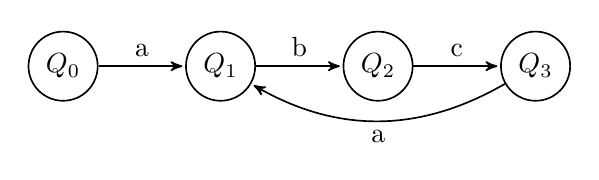
\begin{tikzpicture}[->,>=stealth',shorten >=1pt,auto,node distance=2cm,semithick]
	  \node[state] (A)              {$Q_0$};
	  \node[state] (B) [right of=A] {$Q_1$};
	  \node[state] (C) [right of=B] {$Q_2$};
	  \node[state] (D) [right of=C] {$Q_3$};          
	  \path
(A) edge  node {a} (B)
(B) edge  node {b} (C)
(C) edge  node {c} (D)
(D) edge [bend left]  node {a} (B)
;
	\end{tikzpicture}
  \end{center}
  \end{scriptsize}  
 \caption{\small Four-symbol four-state {\em regular automata} for recognizing the $\{(abc)^n : n \geq 1 \}$ language.}
\label{fig:regautomatae}
\end{figure}

The \strips\ action schema of Figure~\ref{fig:reg-update-rule} models the rule $a,q_0\rightarrow q_1$ of the {\em regular automatae} defined in Figure~\ref{fig:regautomatae}. The full encoding of the {\em automata} of Figure~\ref{fig:regautomatae} produces a total of sixteen \strips\ action schema.

\begin{figure}
\begin{scriptsize}
\begin{lstlisting}
(:action transition-1      ;;; a,$q_0\rightarrow$ $q_1$
  :parameters (?x ?xr)
  :precondition (and (head ?x) (symbol-a ?x) ($q_0$)
                     (next ?x ?xr))
  :effect (and (not (head ?x)) 
               (not (symbol-a ?x)) (not ($q_0$))
               (head ?xr) ($q_1$)))
\end{lstlisting}
\end{scriptsize}
 \caption{\small \strips\ action schema that models the transition $q_0\rightarrow q_1$ of the automata defined in Figure~\ref{fig:regautomatae}.}
\label{fig:regupdate-rule}
\end{figure}

\subsection{Recognition of {\em Turing Machines}}
We analyze now {\em model recognition} when the input set of given set of models represent different {\em Turing machines}.

A {\em Turing machine} is a tuple $\mathcal{M}=\tup{Q,q_o,Q_{\bot},\Sigma,\Upsilon,\square,\delta}$:
\begin{itemize}
\item $Q$ is a finite and non-empty set of machine states with the {\em initial state} $q_0\in Q$ and the {\em terminal states} $Q_{\bot}\subseteq Q$.  
\item $\Sigma$ is the {\em tape alphabet}, a finite non-empty set of symbols with the {\em input alphabet} $\Upsilon\subseteq\Sigma$ (symbols allowed to initially appear in the tape) and the {\em blank symbol} $\square\in\Upsilon$ (the only symbol allowed to occur on the tape infinitely often).
\item $\delta: \Sigma\times (Q\setminus Q_{\bot}) \rightarrow \Sigma\times Q\times\{left,right\}$ is the {\em transition function}. For each pair of tape symbol and non-terminal machine state $\delta$ defines: (1), the tape symbol to print at the current position of the header (2), the new state of the machine and (3), whether the header is shifted {\em left} or {\em right} after the print operation. If $\delta$ is not defined for the current pair of tape symbol and machine state, the machine halts.
\end{itemize}

Figure~\ref{fig:tautomatae} illustrate a seven-symbol six-state {\em Turing Machine} for recognizing the $\{a^nb^nc^n : n \geq 1 \}$ language. The {\em tape alphabet} is $\Sigma=\{a,b,c,x,y,z,\square\}$, the {\em input alphabet} $\Upsilon=\{a,b,c,\square\}$ and the machine states are $Q=\{q_0,q_1,q_2,q_3,q_4,\underline{q_5}\}$ (where \underline{$q_5$} is the only acceptor state).

\begin{figure}
  \begin{scriptsize}
  \begin{center}
	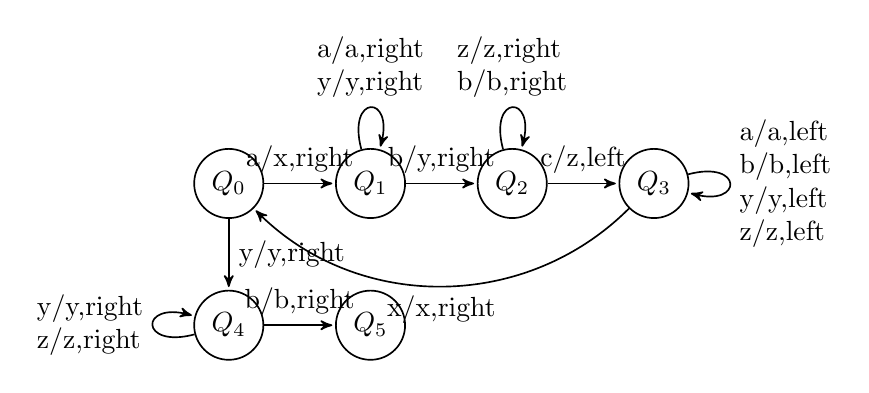
\begin{tikzpicture}[->,>=stealth',shorten >=1pt,auto,node distance=1.8cm,semithick]
	  \node[state] (A)              {$Q_0$};
	  \node[state] (B) [right of=A] {$Q_1$};
	  \node[state] (C) [right of=B] {$Q_2$};
	  \node[state] (D) [right of=C] {$Q_3$};
	  \node[state] (E) [below of=A] {$Q_4$};
	  \node[state] (F) [right of=E] {$Q_5$};                    

	  \path
(A) edge  node {a/x,right} (B)
(B) edge [align=left, loop above] node {a/a,right\\y/y,right} (B)
(B) edge  node {b/y,right} (C)
(C) edge [align=left, loop above] node {z/z,right\\b/b,right} (C)
(C) edge  node {c/z,left} (D)
(D) edge [align=left, loop right] node {a/a,left\\b/b,left\\y/y,left\\z/z,left} (D)
(D) edge [bend left=45] node {x/x,right} (A)

(A) edge  node {y/y,right} (E)
(E) edge [align=left, loop left] node {y/y,right\\z/z,right} (E)
(E) edge  node {b/b,right} (F)
;
	\end{tikzpicture}
  \end{center}
  \end{scriptsize}  
 \caption{\small Seven-symbol six-state {\em Turing Machine} for recognizing the $\{a^nb^nc^n : n \geq 1 \}$ language.}
\label{fig:tautomatae}
\end{figure}


The \strips\ action schema of Figure~\ref{fig:update-rule} models the rule $a,q_0\rightarrow x,r,q_1$ of the {\em Turing Machine} defined in Figure~\ref{fig:tautomatae}. The full encoding of the {\em Turing Machine} of Figure~\ref{fig:tautomatae} produces a total of sixteen \strips\ action schema.

\begin{figure}
\begin{scriptsize}
\begin{lstlisting}
(:action transition-1      ;;; a,$q_0\rightarrow$ x,r,$q_1$
  :parameters (?xl ?x ?xr)
  :precondition (and (head ?x) (symbol-a ?x) ($q_0$)
                     (next ?xl ?x) (next ?x ?xr))
  :effect (and (not (head ?x)) 
               (not (symbol-a ?x)) (not ($q_0$))
               (head ?xr) (symbol-x ?x) ($q_1$)))
\end{lstlisting}
\end{scriptsize}
 \caption{\small \strips\ action schema that models the transition $a,q_0\rightarrow x,r,q_1$ of the Turing Machine defined in Figure~\ref{fig:tautomatae}.}
\label{fig:update-rule}
\end{figure}

With regard to our \strips\ model for {\em Turing Machines}, executions of a {\em Turing Machine} are definable as an action sequence $\tup{a_1, \ldots, a_n}$ that induces the {\em state trajectory} $\tup{s_0, s_1, \ldots, s_n}$ such that $a_i$ ({\small $1\leq i\leq n$}) is applicable in $s_{i-1}$ and generates the successor state $s_i=\theta(s_{i-1},a_i)$. For instance, the execution of the {\em Turing Machine} defined in Figure~\ref{fig:tautomatae} with an initial tape $abc\square\square\square\ldots$ produces the eight-action plan {\small $(a,q_0\rightarrow x,r,q_1)$, $(b,q_1\rightarrow y,r,q_2)$, $(c,q_2\rightarrow z,l,q_3)$, $(y,q_3\rightarrow y,l,q_3)$, $(x,q_3\rightarrow x,r,q_0)$, $(y,q_0\rightarrow y,r,q_4)$, $(z,q_4\rightarrow z,r,q_4)$, $(\square,q_4\rightarrow \square,r,\underline{q_5})$}.

Assuming that the actual applied transitions is unknown means that the observation $\tau$ of the execution of a Turing Machine contains no actions, it is simply a sequence of states $\tau=\tup{s_1, \ldots , s_m}$. Further, assuming that the internal machine state is unknown means that $\tau$ is a $\Phi$-observation and that the $\Phi$ subset does not contain {\small\tt (state-$q$)} fluents, with $q\in Q$ and $q\neq q_0$. Finally, assuming that the values of several tape cells is unknown means that fluents of the kind {\small\tt (symbol-$\sigma$ ?x)} are missing (i.e. unobserved) for some state $s_i\in \tau$ s.t. $1\leq i\leq m$. These facts affects to the a priori probaility of the possible observations.

On the other hand, the model edition for Turing Machines is limited to these subset of possible positive effects: {\tt (head ?xr)} or {\tt (head ?xl)}, {\tt(symbol-$\sigma$ ?x)} with $\sigma \in \Sigma$ and last but not least, {\tt (state-q)} with $q\in Q$. No other positive effects, preconditions, or negative effects are required to be edited. This fact reduces the possible edition operations and affects to the a priori probaility of the possible action models.

\subsection{Results}

\subsection{Conclusions}
\label{sec:conclussions}
The task of {\em model recognition} can also be understood as a classification task where each class is represented with a different planning model and the observed plan execution is the example to classify. With this regard, planning model that is associated to a class is acting as a class prototype that the summarizes all the plan executions that could be synthesized with that model or in other words, all the examples that belong to that class.

In this work we do not assume that the observed agent is acting rationally, like in {\em plan recognition as planning}~\cite{ramirez2012plan,ramirez2009plan}. A related approach is recently followed for {\em model reconciliation}~\cite{Kambhampati:mreconciliation:ijcai17} where model edition is used to conform the PDDL models of two different agents.

Remarkably, the extension of this piece of work to the FOND planning setting~\cite{muise2012improved} is straightforward by simply considering the {\em all-outcomes} determiniztion of the actions with non-determinitic effects~\cite{yoon2007ff}. An interesting research direction is however to understand how to apply our approach to planning models where the planning models include actions with probabilistic effects~\cite{younes2005first}.  

\bibliographystyle{aaai}
\bibliography{planlearnbibliography}

\end{document}
